\subsection{Data and scenarios}
\label{sec:data}

\paragraph{Reference labels.} MMLU-Redux 2.0 \citep{gema2025are} drew 100 questions uniformly at random from each of the 57 MMLU subjects \citep{hendrycks2021measuring}. Annotators then re-checked each question against external sources, independently of any model's output. This gives a sample of benchmark items whose labels were verified without regard to model disagreement, which is exactly what is needed to know the truth that a DR audit would miss. We keep the \nItems{} items whose reference label is determined:
\begin{itemize}
\item items annotated as correct, for which $Y=L$;
\item items annotated as having a wrong ground truth together with a parseable corrected answer.
\end{itemize}
We exclude items with unclear questions or options, no correct answer, multiple correct answers, or an ``expert'' flag, as well as 17 items that could not be matched or parsed (Online Appendix). This leaves \nLabelErrA{} items with a wrong MMLU label (\errRateA\%).

\paragraph{Model predictions.} HELM v1.3.0 \citep{liang2023holistic} publishes per-item predictions of \nModels{} language models on all MMLU subjects (5-shot, joint multiple-choice prompting). We match HELM instances to MMLU-Redux items on question and option text. Outputs that are not a bare option letter are counted as wrong, as HELM does.

\paragraph{Scenarios.} In \emph{Scenario A} the benchmark labels are the original MMLU labels. In \emph{Scenario B} the benchmark's labels are produced by a language model. Such benchmarks exist: the MedCalc-Bench audit of \citet{ye2026scalable} recomputed the test labels with Gemini~2.5~Pro, had a physician review 50 instances sampled from the top of the disagreement ranking, and scored newer models against the recomputed labels, with physician labels substituted on the reviewed subset. We simulate this case by taking one HELM model's answers as $L$; that model is then removed from the evaluated set. We use four labelers: Mixtral 8x7B (the main case), Llama 2 70B, GPT-3.5 Turbo and Qwen1.5 72B. Their label-error rates against MMLU-Redux are \errRateBmin--\errRateBmax\%. In both scenarios the flagger is a single model, or a panel combined by the union rule. We simulate the DR audit exactly: flagged items receive their MMLU-Redux label and all other items keep $L$. Because all reference labels are known, we can also compute every model's true accuracy.

\subsection{What discrepant resolution misses, and whom it favours}
\label{sec:emp-bias}

\begin{table}[t]
\centering
\scriptsize
\begin{tabular}{lrrrrrrr}
\toprule
Labels & Label err.\ (\%) & Hidden $|J|$ & Flagger inflation, pp & Flaggers & Max ranks & Kendall $\tau$ & $P(J)$ / indep. \\
 & & (range) & median [min, max] & favoured & gained & (range) & (median) \\
\midrule
(A) original MMLU & 1.8 & 8--30 & 0.31 [0.15, 0.55] & 7/37 & 3 & 0.99--1.00 & 1.8 \\
\midrule
Mixtral 8x7B & 26.5 & 284--698 & 10.7 [5.2, 12.9] & 33/36 & 25 & 0.80--0.98 & 4.8 \\
Llama 2 70B & 28.9 & 285--753 & 10.9 [5.3, 13.9] & 33/36 & 25 & 0.78--0.97 & 4.4 \\
GPT-3.5 Turbo & 29.6 & 274--754 & 10.3 [5.1, 13.9] & 33/36 & 27 & 0.80--0.97 & 4.3 \\
Qwen1.5 72B & 21.0 & 265--556 & 9.0 [4.9, 10.3] & 32/36 & 13 & 0.88--0.98 & 4.9 \\
\bottomrule
\end{tabular}

\caption{DR audits over all single-model flaggers. ``Hidden $|J|$'' is the number of label errors the flagger reproduces, which therefore stay uncorrected. ``Flagger inflation'' is $\theta^\DR_f-\theta_f$, which equals $\Pn(J)$ (Corollary~\ref{cor:flagger}). ``Flaggers favoured'' counts the flaggers that DR ranks above at least one truly more accurate model. ``Max ranks gained'' is the largest rank improvement of a flagger. ``$P(J)$/indep.'' is the hidden-error rate divided by the rate expected if flagger and label erred independently (Section~\ref{sec:setup}).}
\label{tab:scenarios}
\end{table}

Table~\ref{tab:scenarios} summarises DR audits over every single-model flagger. Table~\ref{tab:flaggersA} details Scenario A for the six strongest flaggers and for union panels. Proposition~\ref{prop:bias} holds exactly for every model, flagger and scenario: our code checks the identity to machine precision.

\paragraph{Scenario A: the original MMLU labels.} With one of the five most accurate models as flagger, a DR audit adjudicates \adjTopFiveMinA--\adjTopFiveMaxA{} items (15--19\% of the benchmark). It finds 80--84 of the \nLabelErrA{} label errors and leaves \hiddenTopFiveMinA--\hiddenTopFiveMaxA{} hidden. Over all \nModels{} possible flaggers, between \hiddenMinA{} and \hiddenMaxA{} label errors stay hidden. The flagger's accuracy is inflated by \inflMinA--\inflMaxA{} percentage points (pp). The hidden-error rate is a median \indepRatioA{} times the rate expected under independent errors.

In this low-noise regime the distortions are small. No strong flagger overtakes a better model, and across all flaggers the largest rank gain is \rankGainA{} places (\favFlaggersA{} of \nModels{} flaggers overtake at least one better model). Panels of the most accurate models shrink the hidden set, but slowly. The top-10 panel still leaves \topTenHiddenA{} hidden errors after adjudicating \topTenAdjA{} items, and the union of all \nModels{} models leaves none but adjudicates \allPanelAdjA{} items (\allPanelAdjPctA\% of the benchmark), little less than a full re-annotation. Smaller panels chosen with hindsight can remove all hidden errors more cheaply, but choosing them requires knowing where the errors are.

\begin{table}[t]
\centering
\scriptsize
\begin{tabular}{lrrrrrrr}
\toprule
Flagger & True rank & Adjudicated & Errors caught & Hidden $|J|$ & Inflation (pp) & Inversions & Flagger-favouring \\
\midrule
Claude 3 Opus & 1 & 802 & 83 & 17 & 0.31 & 0 & 0 \\
GPT-4o & 2 & 819 & 81 & 19 & 0.35 & 0 & 0 \\
GPT-4 (0613) & 3 & 879 & 83 & 17 & 0.31 & 0 & 0 \\
Gemini 1.5 Pro & 4 & 973 & 80 & 20 & 0.37 & 0 & 0 \\
GPT-4 Turbo & 5 & 1045 & 84 & 16 & 0.30 & 0 & 0 \\
Llama 3 70B & 6 & 1075 & 81 & 19 & 0.35 & 0 & 0 \\
\midrule
top-3 panel (union) & -- & 1291 & 87 & 13 & 0.24 & 0 & 0 \\
top-5 panel (union) & -- & 1667 & 88 & 12 & 0.22 & 0 & 0 \\
top-10 panel (union) & -- & 2164 & 93 & 7 & 0.13 & 0 & 0 \\
all models (union) & -- & 5051 & 100 & 0 & 0.00 & 0 & 0 \\
\bottomrule
\end{tabular}

\caption{Scenario A (original MMLU labels, \nLabelErrA{} label errors among \nItems{} items): DR audits with the six most accurate models as single flaggers, and with union panels of the top 3, 5, 10 and all models. ``Inflation'' is the flagger's DR bias; for panels it is the largest bias among panel members, which equals $\Pn(J_G)$ (Proposition~\ref{prop:panel}). ``Inversions'' counts model pairs whose order DR reverses. Online Appendix Table~OA.1 lists all \nModels{} flaggers.}
\label{tab:flaggersA}
\end{table}

\paragraph{Scenario B: a benchmark labelled by a language model.} When the labels come from a language model, hidden errors are common and DR's bias becomes large. Flagger inflation ranges from \inflMinB{} to \inflMaxB{}~pp. Between \favFlaggersBmin{} and \favFlaggersBmax{} of the 36 flaggers are ranked above at least one truly better model, and a flagger gains up to \rankGainBmin--\rankGainBmax{} places, depending on the labeler. The hidden-error rate is \indepRatioBmin--\indepRatioBmax{} times the independence prediction, because language models share their mistakes.

Figure~\ref{fig:sweep} extends this to all \sweepN{} models as labelers. Their label-error rates range from \sweepErrMin\% (\sweepBestLabeler) to \sweepErrMax\%. Even the best labeler gives a median flagger inflation of \sweepBestMedInfl~pp and a largest rank gain of \sweepBestMaxGain. Across labelers, the median inflation ranges from \sweepMedInflMin{} to \sweepMedInflMax~pp, and at least \sweepFavMin{} of the 36 flaggers overtake a better model. The original MMLU labels sit far below all language-model labelers. The two outlying maxima of about 20~pp come from a near-duplicate pair: PaLM~2 Unicorn and Palmyra X v3 give the same answer on \dupAgree\% of items (all but \dupDiffer). When one labels and the other flags, the audit corrects almost nothing.

Figure~\ref{fig:slope}(a) shows one audit: with Mixtral 8x7B labels and Llama~3~70B as flagger, DR inflates the flagger by \llamaInflB~pp and moves it from rank \llamaTrueRankB{} to rank \llamaDrRankB. Figure~\ref{fig:slope}(b) shows that rank gains are largest for flaggers of middling accuracy. Those flaggers have many truly better models to overtake and enough hidden errors to do it.

\begin{figure}[t]
\centering
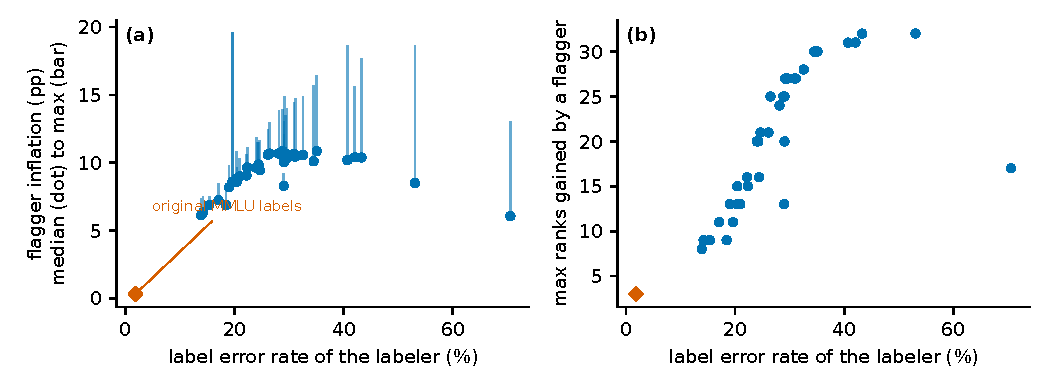
\includegraphics[width=\linewidth]{figures/fig_sweep.pdf}
\caption{Labeler-strength sweep. Each blue point is a benchmark labelled by one of the \sweepN{} HELM models (Scenario B), audited by DR with each of the other 36 models as flagger; the red diamond is Scenario A. (a)~Median flagger inflation (dot) up to the largest (bar). (b)~Largest number of ranks gained by any flagger.}
\label{fig:sweep}
\end{figure}

\subsection{Lock-in}
\label{sec:emp-lockin}

\begin{figure}[t]
\centering
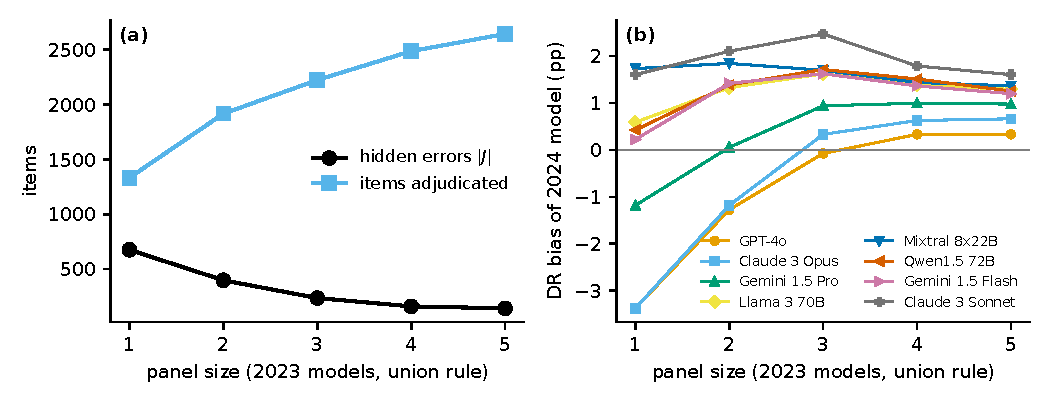
\includegraphics[width=\linewidth]{figures/fig_lockin.pdf}
\caption{Lock-in in Scenario B (Mixtral 8x7B labels). A panel of models released in 2023 cleans the benchmark by DR, and models released in 2024 are evaluated on the result. (a) Hidden errors and adjudicated items as the panel grows (panel order: GPT-3.5 Turbo, Llama 2 70B, Claude 2.1, PaLM 2 Bison, Claude Instant 1.2). (b) DR bias of the 2024 models. With a single flagger, the two strongest 2024 models, GPT-4o and Claude 3 Opus, are each underestimated by a net \lockGptOneB~pp.}
\label{fig:lockin}
\end{figure}

Proposition~\ref{prop:panel}(c) predicts that models built after an audit are penalised on the errors the auditing models share. Figure~\ref{fig:lockin} tests this by cleaning the Scenario B benchmark with models released in 2023 and evaluating models released in 2024. With GPT-3.5 Turbo as the only flagger, \lockHiddenOneB{} label errors stay hidden. GPT-4o answers \lockGptCorrectOneB{} of them correctly and is scored wrong on each, costing it \lockGptCorrectPpOneB~pp. It repeats the wrong label on \lockGptRepeatOneB{} others and is credited for them (\lockGptRepeatPpOneB~pp), so it is underestimated by a net \lockGptOneB~pp. Claude~3~Opus is underestimated by the same net amount (\lockOpusCorrectOneB{} correct answers and \lockOpusRepeatOneB{} repetitions; the two differences coincide). Weaker 2024 models that repeat more of the hidden errors are instead overestimated. Growing the panel to \lockPanelLastB{} models reduces the hidden errors to \lockHiddenLastB{}, but doubles the adjudicated set from \lockAdjOneB{} to \lockAdjLastB{} items. Some bias remains for every 2024 model, now positive, because the surviving hidden errors are the ones most models share. In Scenario A the same experiment leaves \lockHiddenLastA{} hidden errors after adjudicating \lockAdjLastA{} items, and the effect is negligible.

\subsection{A published audit: CoNLL-2003}
\label{sec:emp-conll}

\begin{table}[t]
\centering
\scriptsize
\begin{tabular}{lrrrrrrrrr}
\toprule
 & \multicolumn{2}{c}{Token accuracy (\%)} & \multicolumn{3}{c}{DR bias (pp)} & \multicolumn{2}{c}{Hidden errors} & \multicolumn{2}{c}{Rank} \\
\cmidrule(lr){2-3}\cmidrule(lr){4-6}\cmidrule(lr){7-8}\cmidrule(lr){9-10}
Model & CoNLL++ & DR & total & hidden & disagr. & correct & repeat & true & DR \\
\midrule
RoBERTa-large (J.-B.) & 98.97 & 98.57 & -0.40 & -0.017 & -0.382 & 57 & 49 & 1 & 1 \\
BERT-large (dbmdz) & 98.81 & 98.52 & -0.29 & +0.045 & -0.337 & 42 & 63 & 2 & 2 \\
BERT-large (dslim) & 98.75 & 98.42 & -0.33 & +0.017 & -0.345 & 49 & 57 & 3 & 3 \\
BERT-base (dslim) & 98.65 & 98.38 & -0.27 & +0.045 & -0.317 & 41 & 62 & 4 & 4 \\
DistilBERT (elastic) & 98.28 & 98.00 & -0.27 & +0.060 & -0.332 & 36 & 64 & 5 & 5 \\
Florian (2003) & 97.91 & 97.51 & -0.40 & +0.019 & -0.414 & 39 & 48 & 6 & 6 \\
Chieu (2003) & 97.72 & 97.50 & -0.22 & +0.108 & -0.326 & 25 & 75 & 7 & 7 \\
Klein (2003) & 97.43 & 97.25 & -0.18 & +0.138 & -0.317 & 13 & 77 & 8 & 8 \\
Zhang (2003) & 97.28 & 97.01 & -0.27 & +0.041 & -0.307 & 38 & 57 & 9 & 9 \\
Curran (2003) & 97.13 & 96.87 & -0.26 & +0.054 & -0.315 & 35 & 60 & 10 & 10 \\
Munro (2003) & 97.07 & 96.83 & -0.24 & +0.063 & -0.302 & 34 & 63 & 11 & 11 \\
Carreras (a) (2003) & 97.03 & 96.78 & -0.25 & +0.041 & -0.296 & 27 & 46 & 12 & 12 \\
Mayfield (2003) & 97.02 & 96.78 & -0.25 & +0.093 & -0.341 & 23 & 66 & 13 & 12 \\
Bender (2003) & 96.99 & 96.73 & -0.26 & +0.017 & -0.276 & 43 & 51 & 14 & 14 \\
Carreras (b) (2003) & 96.70 & 96.43 & -0.28 & +0.056 & -0.335 & 25 & 51 & 15 & 16 \\
McCallum (2003) & 96.68 & 96.43 & -0.24 & +0.101 & -0.343 & 24 & 71 & 16 & 15 \\
Hendrickx (2003) & 96.57 & 96.29 & -0.28 & +0.028 & -0.309 & 42 & 55 & 17 & 17 \\
Wu (2003) & 96.46 & 96.16 & -0.30 & +0.088 & -0.391 & 23 & 64 & 18 & 18 \\
De Meulder (2003) & 96.42 & 96.08 & -0.34 & +0.028 & -0.367 & 42 & 55 & 19 & 19 \\
Whitelaw (2003) & 96.14 & 95.84 & -0.30 & +0.050 & -0.350 & 35 & 58 & 20 & 20 \\
Hammerton (2003) & 92.13 & 91.93 & -0.20 & +0.091 & -0.294 & 29 & 71 & 21 & 21 \\
\bottomrule
\end{tabular}

\caption{Re-analysis of the published DR audit of CoNLL-2003 \citep{reiss2020identifying} against the independent full re-check CoNLL++ \citep{wang2019crossweigh}. Items are the \cnItems{} test tokens, labelled with their entity type. ``DR'' is accuracy against Reiss et al.'s resolved labels; ``CoNLL++'' is accuracy against the reference. The DR bias splits exactly into the hidden-error term and a term measuring disagreement between the two relabelings on audited tokens (Remark~\ref{rem:adjudicator}). ``Correct''/``repeat'' count the \cnHidden{} hidden errors on which a model gives the reference label or repeats the original one. Systems marked 2003 are CoNLL-2003 shared-task entries, whose outputs formed one of the audit's flagging ensembles; the others are later public transformer models. Appendix Table~\ref{tab:conllentity} repeats the analysis on entity tokens.}
\label{tab:conll}
\end{table}

The analyses so far simulate audits. We now re-analyse a published one. \citet{reiss2020identifying} audited CoNLL-2003 with three model ensembles. They reviewed the entities on which few ensemble members agreed with the label and the spans that many members proposed but the label lacked, and they corrected some nearby labels they noticed along the way. Their release includes every candidate, every verdict and the corrections. CoNLL++ \citep{wang2019crossweigh} is an independent re-check of every test sentence by two annotators, with a final round where their annotations and the original disagreed; it used no model flags. Reiss et al.\ cite it only to compare error rates, and their candidates come only from their own ensembles. Both files contain the same 46{,}435 test tokens in the same order. We exclude \cnExcluded{} tokens affected by tokenization or sentence-boundary corrections, which CoNLL++ does not make, leaving \cnItems. The original uses IOB1 tags and CoNLL++ uses BIO2.

We therefore take the token as the item and its entity type (none, person, location, organisation, miscellaneous) as the label, so the tag scheme does not matter. The adjudicated set $\Dset$ is every token covered by a span that Reiss et al.\ reviewed or corrected: \cnAdj{} tokens (\cnAdjPct\%), of which \cnIncidental{} were reviewed only incidentally. We apply their label corrections with their own code. The models are the \cnNentrant{} shared-task systems and \cnNhf{} public transformer models (Table~\ref{tab:conll}).

Against CoNLL++, \cnRefErr{} tokens of the original test set have the wrong entity type. Only \cnRefErrIn{} of them lie in the audited set; \cnHidden{} (\cnHiddenPct\%) were never examined. Because the CoNLL++ annotators corrected the existing labels rather than labelling blind, their annotations are anchored towards the original, and \cnHidden{} is probably a lower bound on the hidden errors. The two expert relabelings also disagree on many audited tokens. Reiss et al.\ changed \cnReissChanges{} token types and CoNLL++ agrees with \cnAgreeChanges{} of those changes, leaving \cnDisagreeChanges{} tokens on which the two disagree, more than all the label errors that CoNLL++ finds. We do not know which relabeling is right on those tokens; the same anchoring means that some of them may be errors that CoNLL++ missed. We therefore call the second term of the decomposition the \emph{disagreement term}, not an error of the audit.

Table~\ref{tab:conll} decomposes each model's DR bias exactly. The hidden-error term ranges from \cnHiddenMin{} to \cnHiddenMax~pp. It is positive for all models but RoBERTa-large, the strongest and most recent model, which answers more hidden errors correctly than it repeats. It averages \cnHiddenEntrantMean~pp for the 2003 systems, one of whose ensembles flagged the audit, and \cnHiddenHfMean~pp for the later models. This is consistent with lock-in, although the two ranges overlap. The 2003 systems do not share one bias, as Proposition~\ref{prop:panel}(b) would require of a union panel, because Reiss et al.\ flagged by vote thresholds rather than by the union rule. The disagreement term, from \cnAdjMin{} to \cnAdjMax~pp, dominates the total. Rankings are nearly unchanged. Kendall's $\tau_b$, which accounts for the \cnTies{} tie in the DR ranking, is \cnTau, with \cnNinv{} inversion among the \cnPairs{} pairs, between \cnInvA{} and \cnInvB, which differ by \cnInvGap~pp. This is consistent with \citet{reiss2020identifying}, who report no change in ranking.

Token accuracy is dominated by non-entity tokens, which dilutes every effect. Restricting the items to the \cnEnt{} tokens whose original or reference label is an entity, a subset fixed in advance that contains every label error, the hidden-error term ranges from \cnEntHiddenMin{} to \cnEntHiddenMax~pp and the disagreement term from \cnEntAdjMin{} to \cnEntAdjMax~pp. Kendall's $\tau_b$ is \cnEntTau, with \cnEntNinv{} inversion (\cnEntInvA{} and \cnEntInvB, \cnEntInvGap~pp apart; Appendix Table~\ref{tab:conllentity}). The effects scale with the smaller denominator, but the picture is the same.

Read with Theorem~\ref{thm:ident}, the published audit says less than its point estimates suggest. At an assumed concordant error rate of $0.2\%$, close to the true \cnConcRate\%, the identified interval for the most accurate model is \cnWidthTwo~pp wide. The audit puts \cnPairA{} \cnPairDR~pp ahead of \cnPairB, against \cnPairTrue~pp in truth, and the identified set for that difference contains zero once $\varepsilon\ge\cnPairEpsAmbig$. On this benchmark, then, hidden errors are real (more than a third of the label errors) but move token accuracies by at most \cnHiddenAbsMax~pp. The larger uncertainty comes from disagreement between expert relabelings, which no choice of items to adjudicate can remove.

\subsection{Two-phase estimation}
\label{sec:emp-twophase}

\begin{figure}[t]
\centering
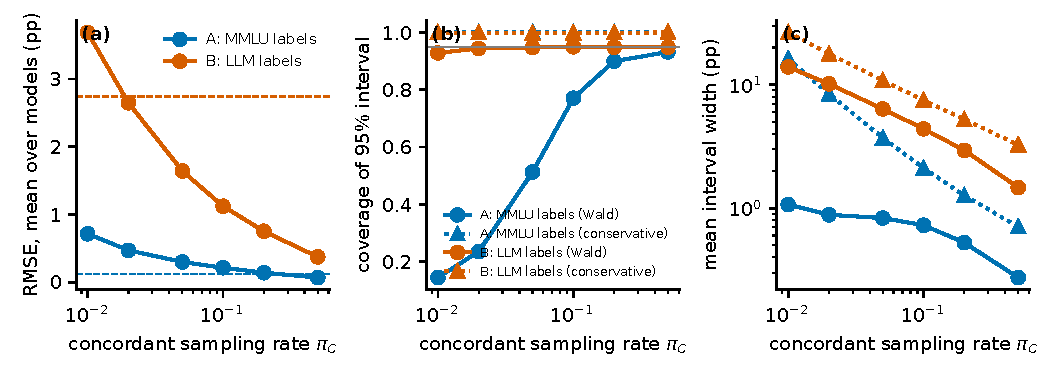
\includegraphics[width=\linewidth]{figures/fig_two_phase.pdf}
\caption{Two-phase estimation with $\pi_\Dset=1$ and concordant sampling rate $\pi_C$, over \reps{} replicates of the phase-two sample (flagger GPT-4o in Scenario A; Llama 3 70B in Scenario B with Mixtral 8x7B labels). (a)~RMSE averaged over models; dashed lines show DR ($\pi_C=0$). (b)~Coverage of nominal 95\% Wald and conservative (Clopper--Pearson) intervals, averaged over models. (c)~Mean interval widths.}
\label{fig:twophase}
\end{figure}

\begin{table}[t]
\centering
\scriptsize
\begin{tabular}{llrrrrrrrr}
\toprule
 & & & & & & \multicolumn{2}{c}{Wald} & \multicolumn{2}{c}{Conservative (CP)} \\
\cmidrule(lr){7-8}\cmidrule(lr){9-10}
Sc. & $\pi_C$ & Adjudicated & $|\text{bias}|$ & RMSE & RMSE$_F$ & cover & width & cover & width \\
\midrule
\multirow{7}{*}{A} & DR ($\pi_C=0$) & 819 & 0.125 & 0.13 & 0.35 & -- & -- & -- & -- \\
 & 0.01 & 865 & 0.014 & 0.72 & 0.80 & 0.145 & 1.07 & 1.000 & 16.22 \\
 & 0.02 & 911 & 0.016 & 0.47 & 0.53 & 0.235 & 0.88 & 1.000 & 8.42 \\
 & 0.05 & 1049 & 0.006 & 0.30 & 0.34 & 0.513 & 0.83 & 1.000 & 3.71 \\
 & 0.1 & 1279 & 0.004 & 0.22 & 0.25 & 0.771 & 0.73 & 1.000 & 2.12 \\
 & 0.2 & 1739 & 0.002 & 0.14 & 0.16 & 0.900 & 0.53 & 1.000 & 1.27 \\
 & 0.5 & 3120 & 0.001 & 0.07 & 0.08 & 0.932 & 0.27 & 1.000 & 0.71 \\
\midrule
\multirow{7}{*}{B} & DR ($\pi_C=0$) & 1170 & 2.740 & 2.74 & 9.72 & -- & -- & -- & -- \\
 & 0.01 & 1213 & 0.094 & 3.68 & 4.15 & 0.929 & 13.92 & 1.000 & 26.48 \\
 & 0.02 & 1255 & 0.040 & 2.65 & 2.95 & 0.944 & 10.15 & 0.999 & 17.81 \\
 & 0.05 & 1382 & 0.029 & 1.64 & 1.85 & 0.947 & 6.37 & 0.999 & 10.81 \\
 & 0.1 & 1595 & 0.028 & 1.12 & 1.29 & 0.950 & 4.39 & 0.999 & 7.49 \\
 & 0.2 & 2020 & 0.017 & 0.75 & 0.85 & 0.949 & 2.94 & 1.000 & 5.24 \\
 & 0.5 & 3296 & 0.007 & 0.38 & 0.42 & 0.949 & 1.47 & 1.000 & 3.26 \\
\bottomrule
\end{tabular}

\caption{Two-phase estimation over \reps{} phase-two replicates; the DR row is deterministic. ``Adjudicated'' is the mean number of adjudicated items. $|\text{bias}|$ and RMSE are averaged over models, in pp; RMSE$_F$ is the flagger's RMSE. Coverage and width refer to nominal 95\% intervals averaged over models.}
\label{tab:twophase}
\end{table}

We simulate the phase-two sample \reps{} times for each concordant sampling rate $\pi_C$, keeping the items fixed and adjudicating all discordant items. Results are in Figure~\ref{fig:twophase} and Table~\ref{tab:twophase}.

The estimator is unbiased, as Theorem~\ref{thm:unbiased} states: the largest Monte Carlo bias over models and sampling rates is \tpMaxBiasA~pp in Scenario A and \tpMaxBiasB~pp in Scenario B. Removing the bias costs some adjudication. In Scenario B, DR's error for the flagger is \drFlagRmseB~pp. With $\pi_C=0.1$ the two-phase estimator reduces it to \tpFlagRmseTenB~pp RMSE, adjudicating on average \tpAdjTenB{} items instead of \tpAdjDRB.

Scenario A shows the limits of the approach when label errors are rare. Only \hiddenGptA{} of the \nCA{} concordant items are mislabelled, so DR's bias is small: \drFlagRmseA~pp for the flagger. At small $\pi_C$ most phase-two samples contain no hidden error at all. The unbiased estimator then has a larger RMSE than DR, and its plug-in variance is often zero, so Wald intervals undercover severely (coverage \tpWaldCovOneA{} at $\pi_C=0.01$ and \tpWaldCovTwentyA{} at $\pi_C=0.2$). The conservative intervals cover in both scenarios (coverage at least \tpCpCovMinA{} in A and \tpCpCovMinB{} in B), at the price of width.

In this regime, then, the honest summary of a DR audit is not a corrected accuracy. It is a corrected accuracy together with an interval wide enough to reflect how little has been learned about concordant items, which is what the simultaneous intervals of Theorem~\ref{thm:simultaneous} provide (Section~\ref{sec:emp-sim}). This is also the regime $m<1/\varepsilon$ of Theorem~\ref{thm:lower}, in which no design can estimate accuracies to better than the order of DR's own bias.

\subsection{Simultaneous exact intervals}
\label{sec:emp-sim}

\begin{table}[t]
\centering
\scriptsize
\begin{tabular}{lrrrrrrrrr}
\toprule
 & & No error & Simult. & \multicolumn{2}{c}{Width, accuracy (pp)} & \multicolumn{2}{c}{Pairs} & \multicolumn{2}{c}{Adjacent pairs (\%)} \\
\cmidrule(lr){5-6}\cmidrule(lr){7-8}\cmidrule(lr){9-10}
Sc. & $\pi_C$ & sampled (\%) & coverage & Thm & CP & width & Wald cov. & certified & wrong \\
\midrule
\multirow{6}{*}{A} & 0.01 & 84 & 1.000 & 11.7 & 16.2 & 21.1 & 0.05 & 6 & 0 \\
 & 0.02 & 69 & 1.000 & 6.5 & 8.4 & 12.2 & 0.09 & 9 & 0 \\
 & 0.05 & 39 & 1.000 & 3.2 & 3.7 & 6.1 & 0.21 & 11 & 0 \\
 & 0.1 & 13 & 1.000 & 2.0 & 2.1 & 3.9 & 0.40 & 18 & 0 \\
 & 0.2 & 2 & 0.985 & 1.3 & 1.3 & 2.6 & 0.59 & 31 & 0 \\
 & 0.5 & 0 & 0.962 & 0.7 & 0.7 & 1.3 & 0.85 & 50 & 0 \\
\midrule
\multirow{6}{*}{B} & 0.01 & 0 & 0.976 & 29.5 & 26.5 & 28.2 & 0.86 & 0 & 0 \\
 & 0.02 & 0 & 0.962 & 25.6 & 17.8 & 27.4 & 0.95 & 0 & 0 \\
 & 0.05 & 0 & 0.959 & 22.0 & 10.8 & 26.0 & 0.95 & 0 & 0 \\
 & 0.1 & 0 & 0.955 & 19.6 & 7.5 & 24.3 & 0.95 & 0 & 0 \\
 & 0.2 & 0 & 0.956 & 16.7 & 5.2 & 21.4 & 0.95 & 2 & 0 \\
 & 0.5 & 0 & 0.953 & 10.2 & 3.3 & 13.3 & 0.95 & 3 & 0 \\
\bottomrule
\end{tabular}

\caption{Simultaneous exact intervals (Theorem~\ref{thm:simultaneous}, $\alpha=0.05$) in the design of Table~\ref{tab:twophase}, over \reps{} phase-two replicates. ``No error sampled'' is the share of replicates in which the concordant sample contains no label error. ``Simult.\ coverage'' is the share of replicates in which every accuracy and every pairwise difference is covered. Widths are means over models (accuracies) and over adjacent pairs of the true ranking. For comparison, ``CP'' is the per-model Clopper--Pearson width and ``Wald cov.'' the range of Wald coverage for the top pairs of Table~\ref{tab:twophase}. ``Certified'' is the share of the \simNadjA{} (A) or \simNadjB{} (B) adjacent pairs whose interval excludes zero; ``wrong'' is the share certified in the wrong direction.}
\label{tab:simultaneous}
\end{table}

Table~\ref{tab:simultaneous} evaluates Theorem~\ref{thm:simultaneous} in the same design as Table~\ref{tab:twophase}. Simultaneous coverage of all accuracies and all pairwise differences is at least \simCovMinA{} in Scenario A and \simCovMinB{} in Scenario B at every sampling rate. No adjacent pair was ever certified in the wrong direction.

In Scenario A, where label errors are rare, the simultaneous intervals for single accuracies are no wider than the per-model Clopper--Pearson intervals, and narrower at small sampling rates (\simWidthOneA{} against \cpWidthOneA~pp at $\pi_\Cset=0.01$). This holds even though they cover all models and pairs at once. At $\pi_\Cset=0.01$ the concordant sample contains no label error in \simNoErrOneA\% of replicates, so the intervals there are those of the procedure in Section~\ref{sec:rule}. For pairwise differences they are the only valid option: Wald intervals for the top pairs cover only \waldPairCovOneA{} of the time at $\pi_\Cset=0.01$. Validity costs resolution, however. Adjacent models in the ranking differ by fractions of a point, so the intervals certify \simCertFiveA\% of adjacent pairs at $\pi_\Cset=0.05$ and \simCertHalfA\% at $\pi_\Cset=0.5$, out of the \simTrueCertA\% that have a strictly positive true difference.

In Scenario B, where hidden errors are common, the intervals remain valid but are wide (\simWidthFiveB~pp at $\pi_\Cset=0.05$), and almost no pair is certified. Here the Wald intervals are both valid and much narrower (Table~\ref{tab:twophase}). This is the division of labour that Proposition~\ref{prop:width} predicts.

\subsection{Allocation at a fixed budget}
\label{sec:emp-alloc}

\begin{table}[t]
\centering
\scriptsize
\begin{tabular}{lrrrrrrrr}
\toprule
 & & & Uniform & \multicolumn{2}{c}{Two-phase ($\pi_\Delta=1$)} & \multicolumn{3}{c}{Neyman} \\
\cmidrule(lr){5-6}\cmidrule(lr){7-9}
Sc. & $B/|\Delta|$ & $B$ & RMSE & RMSE & $\pi_C$ & RMSE & $\pi_\Delta$ & $\pi_C$ \\
\midrule
\multirow{6}{*}{A} & 0.25 & 205 & 0.82 & -- & -- & 0.61 & 0.12 & 0.024 \\
 & 0.5 & 410 & 0.57 & -- & -- & 0.41 & 0.23 & 0.048 \\
 & 1 & 819 & 0.38 & -- & -- & 0.27 & 0.46 & 0.095 \\
 & 1.25 & 1024 & 0.33 & 0.33 & 0.044 & 0.23 & 0.58 & 0.119 \\
 & 1.5 & 1228 & 0.30 & 0.23 & 0.089 & 0.20 & 0.70 & 0.143 \\
 & 2 & 1638 & 0.25 & 0.15 & 0.178 & 0.15 & 0.93 & 0.191 \\
\midrule
\multirow{6}{*}{B} & 0.25 & 292 & 2.55 & -- & -- & 2.31 & 0.10 & 0.041 \\
 & 0.5 & 585 & 1.75 & -- & -- & 1.58 & 0.20 & 0.083 \\
 & 1 & 1170 & 1.16 & -- & -- & 1.03 & 0.40 & 0.165 \\
 & 1.25 & 1462 & 1.00 & 1.38 & 0.069 & 0.88 & 0.50 & 0.206 \\
 & 1.5 & 1755 & 0.88 & 0.94 & 0.138 & 0.76 & 0.60 & 0.248 \\
 & 2 & 2340 & 0.70 & 0.61 & 0.275 & 0.59 & 0.80 & 0.330 \\
\bottomrule
\end{tabular}

\caption{RMSE (pp, exact design variance averaged over models) at expected budget $B$ adjudications, expressed as a multiple of the DR budget $|\Dset|$. Designs: uniform random sampling of all items; two-phase with every discordant item adjudicated ($\pi_\Dset=1$, only possible when $B>|\Dset|$); and the Neyman allocation of Proposition~\ref{prop:neyman}, computed with oracle stratum error rates.}
\label{tab:allocation}
\end{table}

Table~\ref{tab:allocation} compares three unbiased designs at equal expected budget. The Neyman allocation is always best. At the DR budget ($B=|\Dset|$) it attains an RMSE of \allocNeyOneA~pp in Scenario A, against \allocUnifOneA~pp for uniform sampling, and \allocNeyOneB{} against \allocUnifOneB~pp in Scenario B. It adjudicates only \allocNeyPiDOneA{} (A) and \allocNeyPiDOneB{} (B) of the flagged items and spends the rest of the budget on concordant items.

The common practice of adjudicating every flagged item first is not efficient for estimation. In Scenario B, at budgets up to $1.5|\Dset|$, it is worse than ignoring the flags altogether and sampling uniformly. The informative-error rates are $e_\Dset=\eDA$ and $e_\Cset=\eCA$ in A, and $e_\Dset=\eDB$ and $e_\Cset=\eCB$ in B. Their square roots set the optimal ratio of sampling rates. The oracle rates are unknown in practice, so these numbers are an upper bound on the achievable gain. Estimating the stratum error rates from adjudications in the same sample makes the design outcome-dependent, so the variance formula of Theorem~\ref{thm:unbiased} does not apply as stated (Section~\ref{sec:twophase}); rates carried over from earlier audits avoid this, and we do not quantify how much of the gain either approach recovers.

\subsection{Sensitivity analysis of a DR audit}
\label{sec:emp-sens}

\begin{figure}[t]
\centering
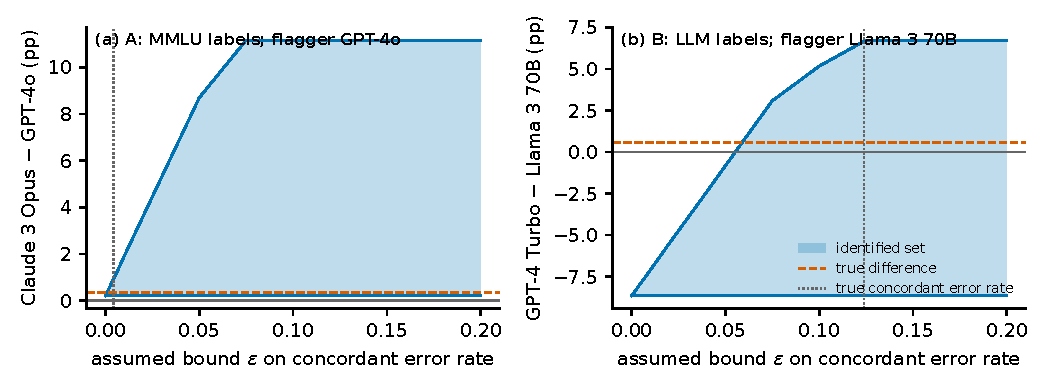
\includegraphics[width=\linewidth]{figures/fig_sensitivity.pdf}
\caption{Sharp identified sets (Theorem~\ref{thm:ident}) for the accuracy difference between a model and the flagger, as a function of the assumed bound $\varepsilon$ on the label-error rate among concordant items. The dashed line marks the true difference and the dotted line the true concordant error rate. The DR value is always the lower endpoint (Corollary~\ref{cor:advantage}).}
\label{fig:sensitivity}
\end{figure}

Figure~\ref{fig:sensitivity} applies Theorem~\ref{thm:ident} to two DR audits as a reader of a published audit would, using only the DR data and an assumed $\varepsilon$.

In Scenario A (flagger GPT-4o), DR reports that Claude~3~Opus is \sensPairDRA~pp more accurate than the flagger; the truth is \sensPairTrueA~pp. Because DR understates advantages over the flagger, the sign of this comparison is identified for every $\varepsilon$.

In Scenario B (flagger Llama~3~70B), DR places GPT-4~Turbo \sensPairDRBabs~pp below the flagger, whereas GPT-4~Turbo is in fact \sensPairTrueB~pp more accurate. For every $\varepsilon$ up to 0.05 the identified set lies entirely below zero, so a reader who trusts a concordant error rate of a few percent would accept the flagger's lead. The set first contains the true difference at $\varepsilon=\sensEpsCoverB$, while the true concordant error rate is \sensTrueRateB. Sensitivity analysis therefore protects a reader only if the assumed $\varepsilon$ is realistic, and DR data cannot tell the reader what is realistic. That is the argument for sampling concordant items. Online Appendix Table~OA.2 reports per-model bounds.

\paragraph{The rate in $m$.} The empirical RMSE of the flagger's estimate (Llama~3~70B, Scenario B) is within a factor of \rateRatioMin--\rateRatioMax{} of the design standard error~\eqref{eq:upper} at every $m$ from 10 to 1{,}000, confirming the $m^{-1/2}$ rate; the lower bound of Theorem~\ref{thm:lower} has the same slope (Online Appendix Figure~OA.1).
